\documentclass[english]{article}
\usepackage[
 %work, %--- activate temporarily to visualise the type area while fine tuning the poster composition
 ,cursor
 ]{KITposter}
 
%Custom packages needed
\usepackage{siunitx}
\usepackage{pgfplots}
\pgfplotsset{compat=newest}
\usepgfplotslibrary{fillbetween}
\usepackage{tikzscale}
\usepackage{tabularx}
\usepackage{enumitem}
\usetikzlibrary{shapes.geometric}
\usetikzlibrary{arrows.meta}

 
\title{Time-Resolved Measurements of Transverse Beam Excitation in an Electron Storage Ring}
\author{\underline{M.-D. Noll}\thanks{marvin-dennis.noll@kit.edu}, E. Bründermann, M. Caselle, E. Huttel, J.~L. Steinmann and A.-S. Müller}
\institute{
\includegraphics[height=6cm]{KARA}}

\footline{\small%
\begin{tabularx}{\linewidth}{p{0.15\linewidth} X p{0.15\linewidth} p{0.09\linewidth}}
     \textbf{Contact} \newline
	 *Marvin-Dennis Noll -- \url{marvin-dennis.noll@kit.edu}\newline Institute for Beam Physics and Technology\newline\url{www.ibpt.kit.edu} \newline Karlsruhe, Germany &
	 \textbf{References} \newline
	 {\footnotesize\begin{enumerate}[nosep,label={[}\arabic*{]}]
	 \item S. Hiramatsu et. al., ``Measurement of Small Beam Size by the Use of SR Interferometer'',\newline in Proc. Particle Accel. Conf., New York, USA, 1999, pp. 492-494
	 \item L. Torino and U. Iriso, ``Transverse beam profile reconstruction using synchrotron radiation interferometry'',\newline \texttt{doi: 10.1103/PhysRevAccelBeams.19.122801}
	 \item M. Patil et al., ``Application of KALYPSO as a diagnostic tool for beam and spectral analysis'',\newline \texttt{doi: 10.18429/JACoW-IPAC2021-WEPAB331}
	 \end{enumerate}} &
	  \textbf{Acknowledgments} \newline 
	  M.-D. Noll acknowledges of the KIT IBPT mechanical engineering department and the mechanical workshop staff" &
	  \textbf{Conference} \newline
	  \raisebox{-4.5cm}{\begin{minipage}[t]{1cm}
\includegraphics[width=8cm]{ibic25.png}\\
	  \textbf{}\end{minipage}}\\
\end{tabularx}
}                  

\def\boxheight{200mm}           
\def\boxsep{6mm}    
\begin{document}
	\maketitle
	\vspace{-40mm}
	
	\begin{boxgrayw}[\boxheight]{Motivation}{}
	\begin{itemize}
		\item Transverse modulation can increase beam size, thus reducing intra-beam scattering
		\item KARA vertical beam size too small for crotch absorber set diffraction limit
		\item Use double slit setup to convert size changes to contrast modulation\textsuperscript{[1]}
		\item Sample these changes with fast (turn-by-turn) line camera KALYPSO\textsuperscript{[2]} to distinguish mere \textit{position} modulation from desired \textit{size} blow-up
	\end{itemize}
\end{boxgrayw}
\begin{boxgray2w}[\boxheight]{Measurement and Excitation Setup at KARA}{}
	\begin{minipage}{250mm}
		\includegraphics[height=170mm]{img/aufbau2.tikz}
	\end{minipage}
\end{boxgray2w}
\vskip\boxsep
\begin{boxgray3w}[\boxheight]{Vertical Profile Measurements with/without Excitation(Sine, 11~W, 460~kHz), No Double Slit}{}
	\includegraphics[height=80mm,width=360mm]{img/u.tikz}\;
	\includegraphics[height=80mm,width=360mm]{img/m1.tikz}
	
	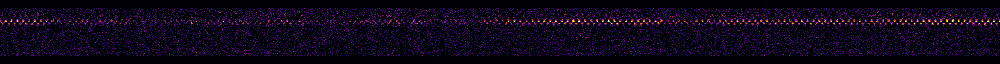
\includegraphics[height=95mm,width=726mm]{img/diff.tikz}\;
\end{boxgray3w}
\vskip\boxsep
\begin{boxgrayw}[\boxheight]{Spectral Analysis}{}
	\includegraphics[height=140mm,width=220mm]{img/spect3.tikz}
	\begin{itemize}
		\item Calculate Periodograms of Pixel no. 40
		\item Modulation and betatron tune detectable
	\end{itemize}
\end{boxgrayw}
\begin{boxgrayw}[\boxheight]{Planned Optimizations}{}
	\begin{itemize}
		\item Optimizing double slit geometry
		\item Calibrate KALYPSO to absolute units
		\item Spectral response used to match double slit and optical bandpass filter
		
		\includegraphics[width=210mm,height=120mm]{img/spectralResponseKalypso.tikz}
	\end{itemize}
\end{boxgrayw}
\begin{boxgrayw}[\boxheight]{Summary and Outlook}{}
	\begin{itemize}
		\item Detector and Modulation setup successfully commissioned
		\item First test show working modulation scheme but double slit measurements not possible due to (radiation-) damaged optics
		
		\vspace{5mm}
		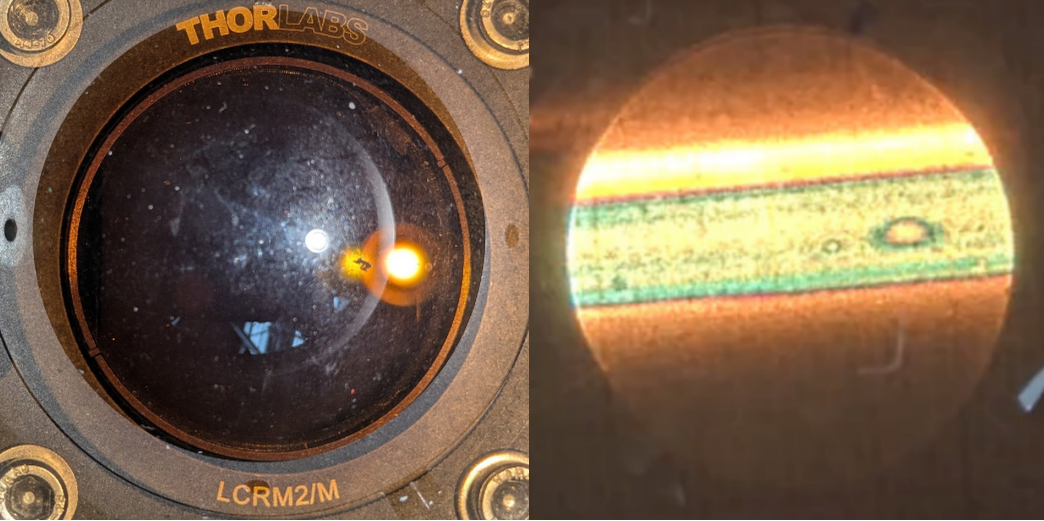
\includegraphics[width=150mm]{img/mirrorAndWindow.png}
		\item Mirror and windows need to be replaced
	\end{itemize}
\end{boxgrayw}

%\tikz[remember picture, overlay] {%
	%\draw [red,line width=0.1mm]
	%(-4,-87.33) rectangle (80.05,31.5);
%}%
	
\end{document}
